

\chapter{Related works}
\label{c:related-works}

In this chapter, we briefly introduced the related techniques used in our system. In section 2.1, we describe basic concept of Internet of Thing. In section 2.2, we introduce the steaming protocols we usually used in streaming. In section 2.3, we present the operation mechanism of a protocal, MQTT.

\section{IOT}

\if 0
\bibliography{thesis}
\graphicspath{{./figsrc/}}
\fi

Internet of Thing, also known as IOT, is a system of network that decribes physical objects with sensors, processing ability, software and variety of computing device, whose power of computation are often worse than normal computers and only served for specific tasks, instead of general propose. For example, connect, collect and exchange data with other devices and systems over the internet or other communication protocols~\cite{iot-intro-01}. Fig.~\ref{fig:iot-intro-02} shows a schematic diagram of IOT system that the structure of the Internet of Things can be divided into three layers. First layer, sensing layer, is consisted of various IOT devices that are responsible for collecting data from field and controlling physical devices that is manully commanded by human or automatically executed. Second layer, network layer, the data that's collected by all of these devices needs to be transmitted and processed. That's the network layer's job. It connects these devices to other smart objects, servers and network devices. It also handles the transmission of all of the data. Third layer, application layer, is what user interacts with. It's responsible for delivering applicaion specific services to the user of overall hub that collates the data collected by the sensing layer and makes analysis or notifies users or gives control commands. This can be a smart home implementation, for example, where users tap a button in the app to turn on a coffee maker.

\begin{figure}[H]
    \centering
    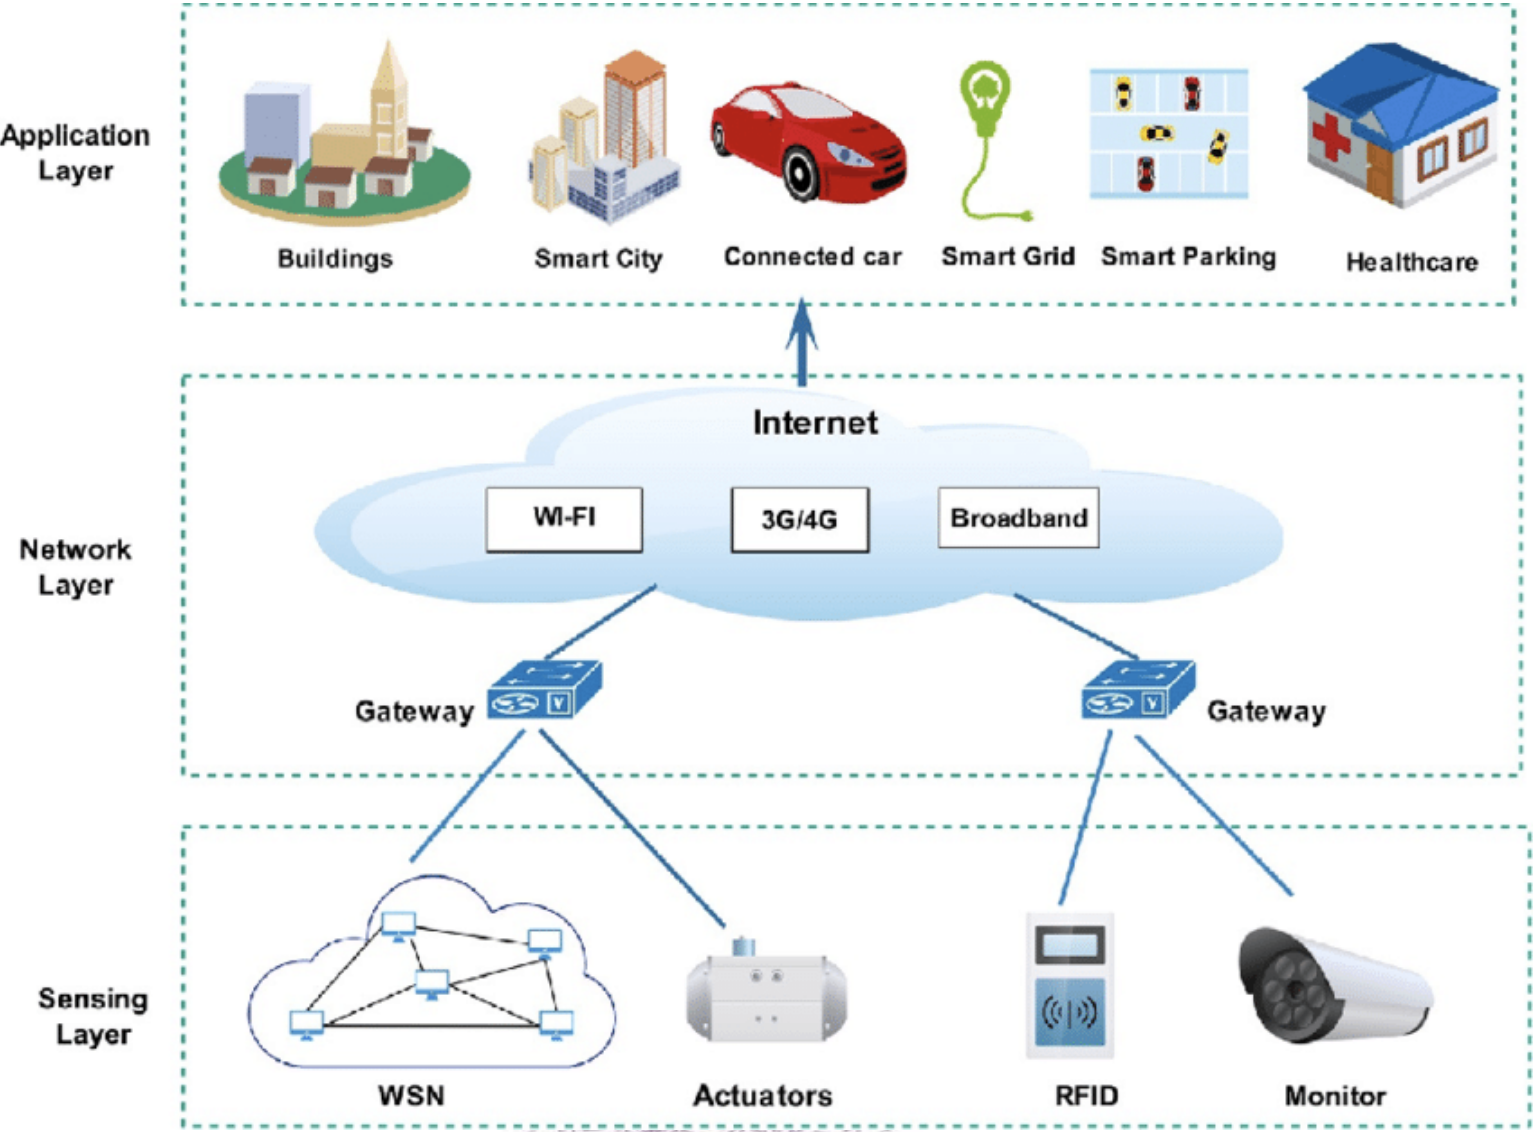
\includegraphics[width=\textwidth]{figsrc/iot-intro.png}
    \caption{The architecture of the Internet of Things system~\cite{iot-intro-02}\label{fig:iot-intro-02}}
\end{figure}

\section{Streaming Protocols}
Streaming Protocols is a set of rules for transmitting multimedia files between 2 communication systems. It defines how your video files will be broken into small data packets and the order in which they'll be transmitted over the internet.
In this sections, we gonna enumerate two frequently used protocols, and describe its pros and cons to determine which one we will choose for IP cam.

First steaming protocol, RTSP, also known as Real Time Streaming Protocol, is an application-level network protocol which are designed for multiplexing and packetizing multimedia transport streams(e.g. interactive mediam video and audio). RTSP was designed and researched by RealNetworks, Netscape~\cite{rtsp-intro-01} and Columbia University~\cite{rtsp-intro-02}. RTSP is widely apllied in such system of entertainment and communications to control straming media servers. The protocol itself is applied for building and controlling media sessions between endpoints. Pros of RTSP is that users can continue to watch a stream while it's still downloading video. Cons is that it isn't widely used for boardcasting multi-media via internet. 

Second, RTMP, also known as Real-Time Messaging Protocol, is a usual protocol for live or on-demand video streaming developed by Macromedia~\cite{rtmp-inventor}. It is initially designed for a stable connection between media server and flash player. Pros of RTMP is that it is good at boardcasting multi-media with stable conneciton. Cons of RTMP is that it isn’t compatible with HTML5 players. So if you want to watch video, you often need to install addtional protocol to support it, such as HLS.

We can summary that RTMP is good at broadcasting while RTSP is good at localized streaming. Both RTMP and RTSP are designed for efficient and low-latency streaming of video files. At last, we choose RTMP for our streaming protocol due to the usage of our IOT platform is to boardcasting. Additionally, we need to know the IP of the camera in order to establish connection with camera by RTSP. This cause another problem that it is time consuming and expensive to apply  a static IP in Taiwan. And if we want to use dynamic IP then we need to use other techniques such as port forward or VPN to access to camera which is also time comsuming. RTMP don't have this disadvantage since live stream of camera will push to a single steaming server as shown in fig.~\ref{fig:rtmp-data-flow}. What we have to do is only need to know the IP and sercuriy setting of the server then we can access to the stream we want. The difficuly to establish a camera streaming is far easier than RTSP.

\begin{figure}[H]
    \centering
    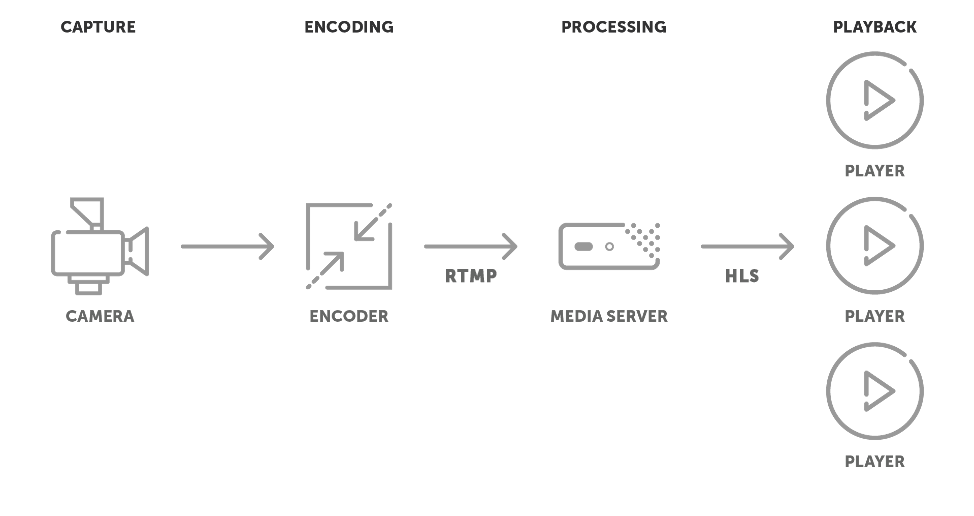
\includegraphics[width=\textwidth]{figsrc/rtmp-data-flow.png}
    \caption{Data flow of RTMP streaming~\cite{rtmp-intro-01}.\label{fig:rtmp-data-flow}}
\end{figure}

\section{MQTT}
Message Queuing Telemetry Transport, also known as MQTT~\cite{mqtt-intro} is a TCP level communication protocol. It is designed for low computing power of hardware devices and poor quality of internet environment and used for transmission between IOT devices. MQTT is a publish–subscribe pattern~\cite{pub-sub} where senders of messages, called publishers, do not program the messages to be sent directly to specific receivers, called subscribers, but instead categorize published messages into topics without knowledge of which subscribers, if any, there may be. Similarly, subscribers express interest in one or more topics and only receive messages that are of interest, without knowledge of which publishers, if any, there are. Information is organized in a hierarchy of topics. When a publisher has a new item of data to distribute, it sends a control message with the data to the connected broker. The broker then distributes the information to any clients that have subscribed to that topic. Fig.~\ref{fig:mqtt-data-flow} show the architecture of an IOT device using MQTT communication. 

\begin{figure}[H]
    \centering
    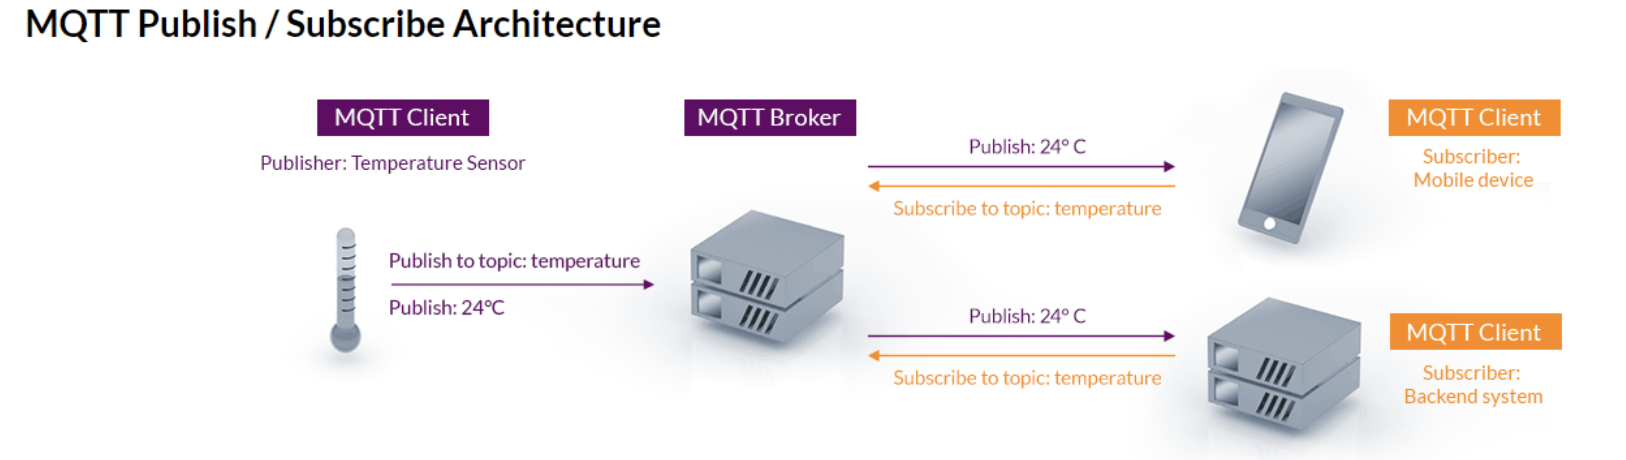
\includegraphics[width=\textwidth]{figsrc/mqtt-data-flow.png}
    \caption{Data flow of MQTT communication~\cite{mqtt-data-flow}\label{fig:mqtt-data-flow}}
\end{figure}

\section{Related video data set}
There were some publication that collected video dataset. For example, ~\cite{video-set-01} contains tens of hours of videos for video grounding and action recognition, and 33000 frames for annotating pose estimation. They collected these data by animal enthusiasts and professionals; ~\cite{video-set-02} collected video from youtube. They used these dataset to detect camouflaged objects in videos. ~\cite{video-set-03} collected chicken data by manual recording from June 10–12, 2019, from 9:00 to 17:00. They transformed chicken videos into pictures to train chicken behavior classification. ~\cite{video-set-04} is similar as ~\cite{video-set-03}. They also collected data by manual recording for cattle recognition. We see that ~\cite{video-set-01} is extremely laborious because they need to collect various field of data to cover extensive range of environmental variations. Compared to ~\cite{video-set-03} and ~\cite{video-set-04}, these researches aimed at analyzing more specific species, so the loading for collecting data was much easier. However, we can find that these researches are lack of automatic collecting service. 

\section{Related data collecting streaming system}
We will enumertate other related data collecting systems in this section and compare the difference of characteristic between us and others.

In agriculture research, there are two type of device which can help crop and stock farmer to monitor and collect image data, Unmanned Aerial Vehicles(UAVs)~\cite{uav-wiki}, or more commonly known as drones and Stationed ground-based surveillance and monitoring system as shown in Fig.~\ref{fig:uav} and Fig.~\ref{fig:cctv_camera}. Both of these systems share many similarities. In summary, there are much more efficient than human beings in capturing and storing data. Both have some disadvantages. For drones, law limitation, expensive cost, safety, weather dependent, vulnerable and considerable pilot training etc. are its shortage. For ground-based monitoring system, limitation of movement and less freedom compared to UAVs are its shortage. We choose ground-based system because it meet most of our need to monitor and collect data. Because it is cheaper compared to UAV and UAV is mush more harder to train pilot since we don't need to train peeple to pan and tilt camera.

\begin{figure}[H]
    \centering
    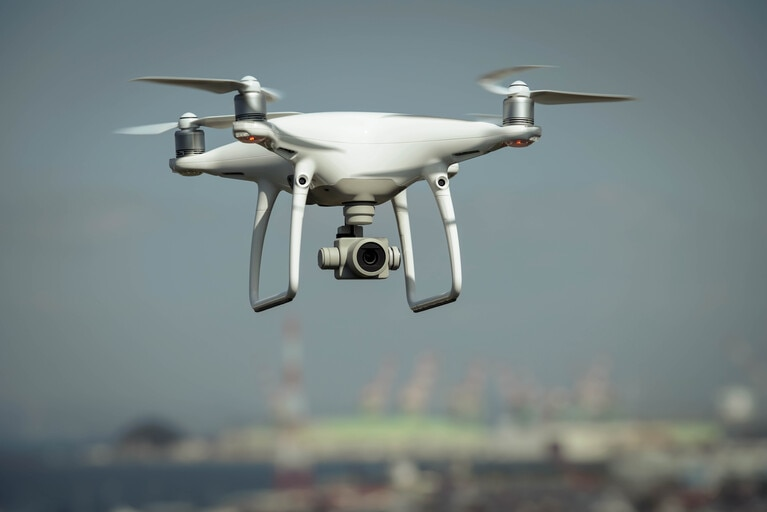
\includegraphics[width=\textwidth]{figsrc/uav.jpeg}
    \caption{Unmanned aerial vehicle is flying in the sky\label{fig:uav}}
\end{figure}


\begin{figure}[H]
    \centering
    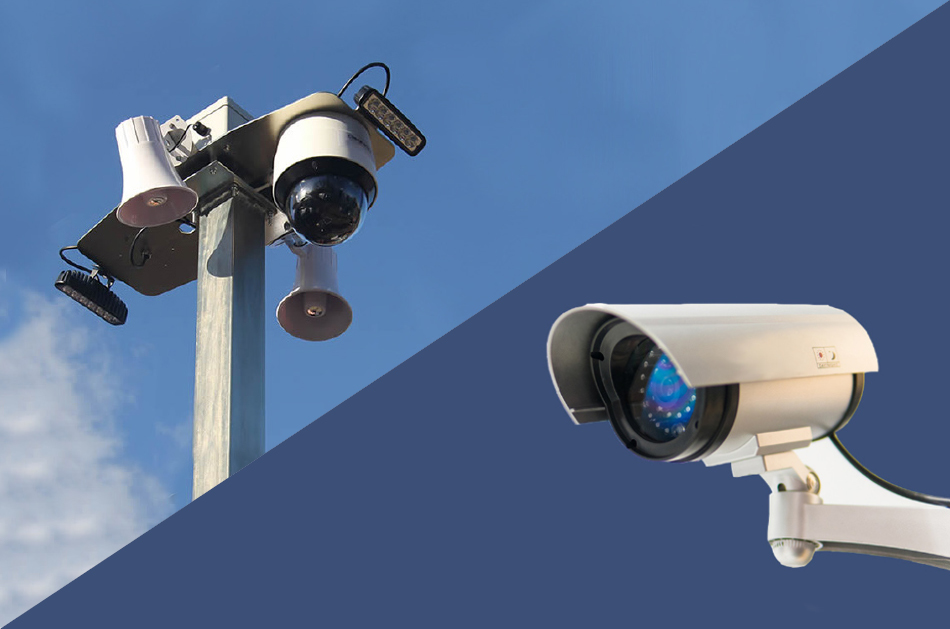
\includegraphics[width=\textwidth]{figsrc/cctv_camera.jpeg}
    \caption{CCTV camera is monitoring the field\label{fig:cctv_camera}}
\end{figure}

In ground-based monitoring system, they usually have 4 parts, cameras, storage, monitors and internet as shown in Fig.~\ref{fig:cctv_system}. Cameras are located at the place that we wish to monitor. The network connects other 3 parts together. It enable camera send live streaming to storage and monitoring station and share with other advanced services.

\begin{figure}[H]
    \centering
    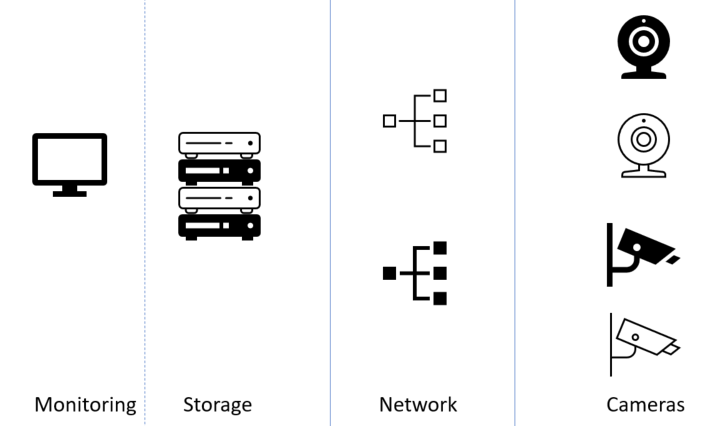
\includegraphics[width=\textwidth]{figsrc/cctv_system.png}
    \caption{Basic components of a CCTV System\label{fig:cctv_system}}
\end{figure}

\subsection{GenBest Technology digital video recording system}
GenBest company~\cite{genbest-LTD} provides the most common traditional system we can find in our daily life. It has basic function for monitoring the specific field. It can see all live stream locally and remotely from internet such as web browser and access history stream which is stored in a local digital video recorder. Due to storage limit, it use technique called loop recording. To achieve never-ending recording, Loop recording will erase the previously recorded material and replacing it with the new content if the disk storage is full. Fig.~\ref{fig:genbest_system} shows the system overview of the whole system. At last, they can improve service by updating software instead of hardware.

\begin{figure}[H]
    \centering
    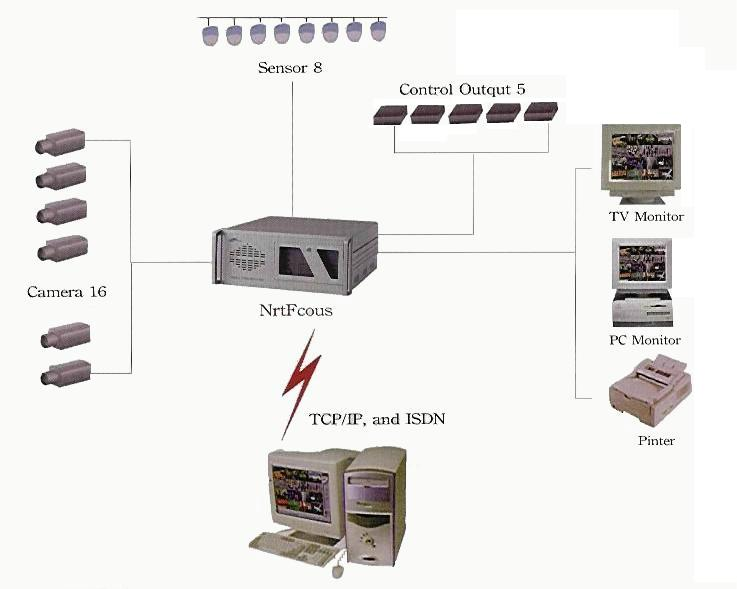
\includegraphics[width=\textwidth]{figsrc/genbest_system.jpeg}
    \caption{Monitoring system overview of GenBest\label{fig:genbest_system}}
\end{figure}

\subsection{Luda farm}
Luda farm~\cite{luda-farm} provides farmers across the world products and services that make everyday work easier, safer and more efficient by IOT system as shown in Fig.~\ref{fig:luda_overview}. This system not only have most of the services of GenBest but also combined with IOT tech. such as sensors and apps in order to fulfill multiple requirement. For data collecting and monitoring perspective, as shown in Fig.~\ref{fig:Luda_farm_cctv}, different to previous system, they not only have usual recording function to monitor animal but also use event triggered record by motion detection for criminal activity. And they have ptz doom cameras for better vision for the field. Furthermore, they have various type of cameras(e.g. doom, bullet and ptz camera etc.) to choose for different purposes and budgets.

\begin{figure}[H]
    \centering
    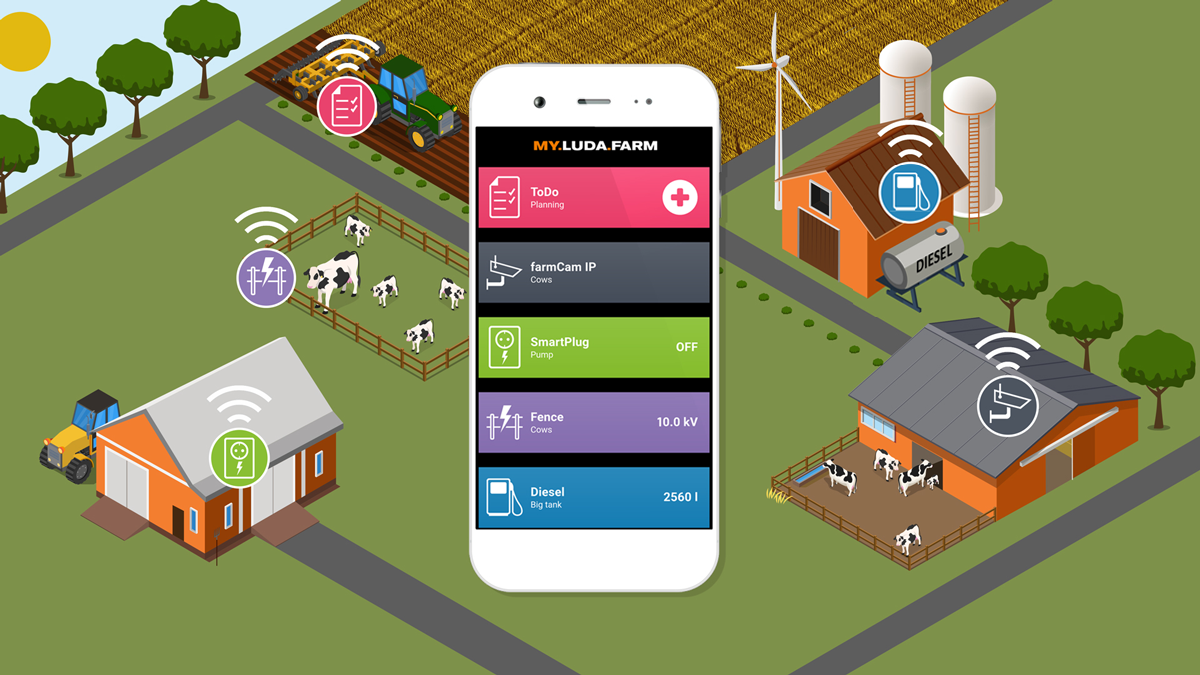
\includegraphics[width=\textwidth]{figsrc/luda_overview.png}
    \caption{Overview of Luda farm system\label{fig:luda_overview}}
\end{figure}

\begin{figure}[H]
    \centering
    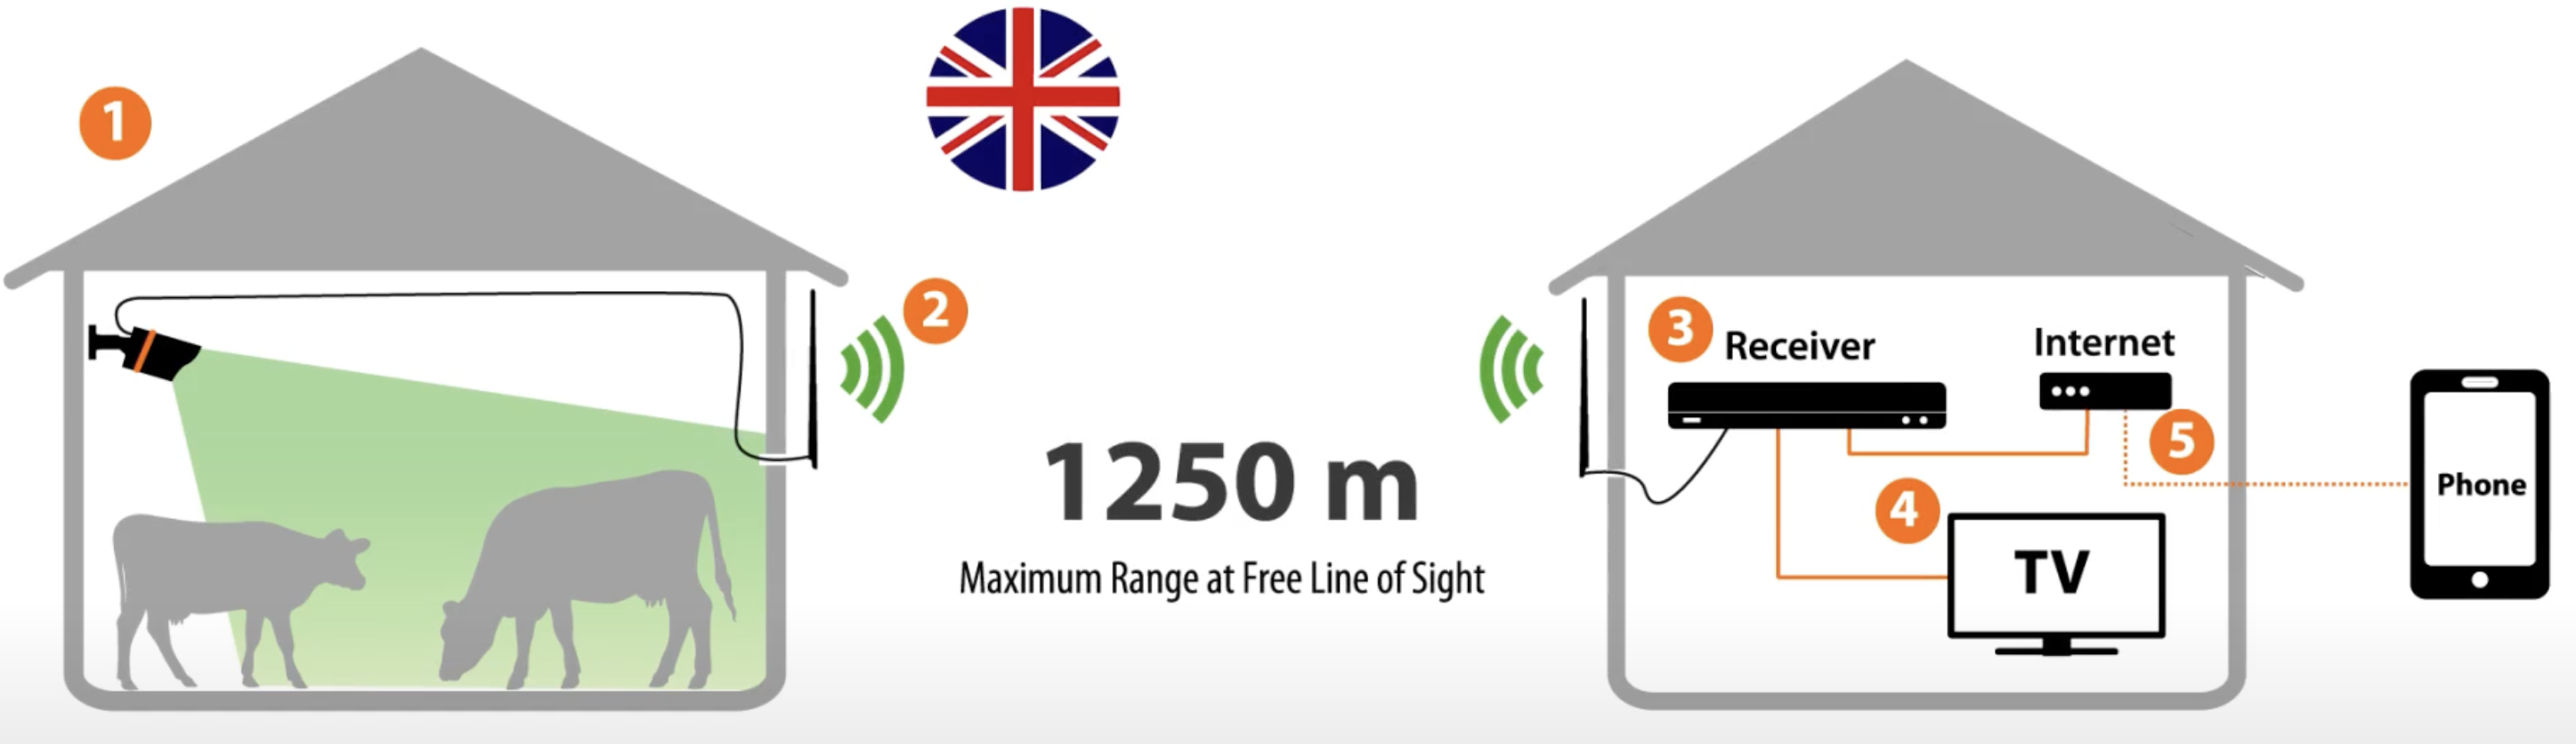
\includegraphics[width=\textwidth]{figsrc/Luda_farm_cctv.png}
    \caption{Overview of Luda farm CCTV system\label{fig:Luda_farm_cctv}}
\end{figure}

\subsection{Speices recognition for wild animal}
They~\cite{wildlife-paper} use camera-trap technologies to monitor wild animals since some of wild animals are afraid of human. It is hard to capture these kind of animals when there are human nearby. The images captured by the camera traps are triggered by a motion sensor and send to AWS cloud for annotating. As shown in Fig.~\ref{fig:wild-animal-paper-1}, They use AWS cloud service as computing and annotating resource and send data to private NAS  which stores all of the post-process image data. At last, they use these data to traing and test their AI model.

\begin{figure}[H]
    \centering
    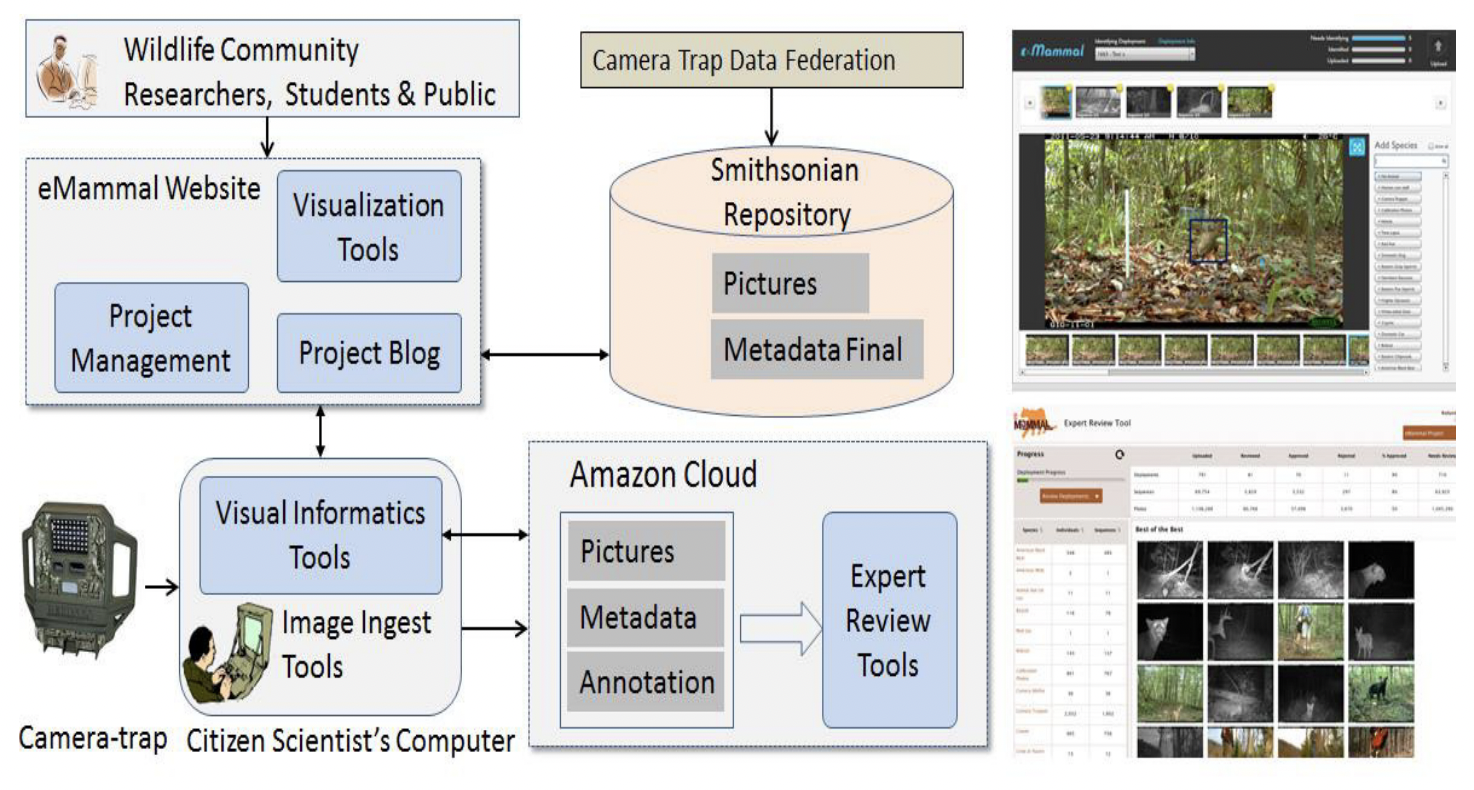
\includegraphics[width=\textwidth]{figsrc/wild-animal-paper-1.png}
    \caption{The framework of eMammal cyber-infrastructure\label{fig:wild-animal-paper-1}}
\end{figure}


We can find out that each system has its benefits and limitations. Our system has camera that can control its degree remotely through internet by 180 vertical and 360 horizontal degree. It have 3 recording types. First, event triggered will send MQTT command to start recording process when specific event happened. Second, we can set a specific timing to trigger recording process. Third, User can click button in Smart Farming Platform webpage to start record manually. Our system use AWS cloud service to achieve central management. Improve storage limit by AWS S3~\cite{aws-s3} and software extensibility by AWS Lambda~\cite{aws-lambda} and Greengrass~\cite{aws-greengrass}.

\begin{table}[H]
    %\hspace{-.5in}
    \resizebox{\textwidth}{!}{
        \begin{tabular}{|c|c|c|c|c|}
            \hline
            {\bf } & {\bf GenBest Tech.} & {\bf Luda farm} & {\bf Wild animal recognition} & {\bf Ours} \\
            \hline
            Camera control flexibility & X & \thead{PTZ, 180 vertical \\ and 360 horizontal}  & X & \thead{PTZ, 180 vertical \\ and 360 horizontal} \\
            \hline
            Agility of dynamic record & X & Event triggered & Event triggered & Event triggered, time scheduling \\
            \hline
            Multi-field capability & X & V & V & V \\
            \hline
            Cloud based management & X & Limited & AWS service support & AWS service support \\
            \hline
            Software extensibility & Limited & Unknown & Cloud based extendable & Cloud based extendable \\
            \hline
            % Curvature & deterministic & height/width ratio of sine curve \\
            % \hline
            % Typeset Emulation & both & \parbox[c]{9cm}{gap width, maximal height and variance of vertical shift} \\
            % \hline
            % Line Interruptions & random & \parbox[c]{9cm}{interruption frequency, maximal width and variance of gap width} \\
            % \hline
            % Thickness Variation & random & \parbox[c]{9cm}{Markov chain stationary distribution and inertia factor} \\
            % \hline
            % $y$-variation & random & \parbox[c]{9cm}{Markov chain stationary distribution and inertia factor} \\
            % \hline
            % Degradation & random & \parbox[c]{9cm}{emulating local distortions suggested by Kanungo et al.} \\
            % \hline
            % White Speckles & random & \parbox[c]{9cm}{speckle frequency, random walk length and smoothing factor} \\
            % \hline
        \end{tabular}
    }
    \caption{Monitoring-system comparison.\label{table:Monitoring-system}.}
\end{table}





% \section{Streaming control and photo collect scheduling
%  system}
% In Chapter 1, we mentioned about previous work had establish a IOT system to solve the problem we meet in agriculture and we will focus on function related to IP cam. And we also briefly introduce how the streaming system work. At last we pointed out the improvement that could be made. We gonna introduce the detail of the system structure they made in this section. 

% Fig.~\ref{fig:Previous-IPcam-system-chart} is the architecture of the entire streaming system. As mentioned in chapter 1, Streaming system aims to collect data and upload to cloud storage to provide training data for AI model. Additionally, system provides live streaming for user to observe on-site situation and allow user to control camera for rotation, zooming and taking photo manually. Their system architecture is divided into several parts, Front-end, Back-end, Edge-device. 
%     \subsection{Front-end}
%     Front end server is responsible for providing interface to user, including live streaming, control and time scheduling UI. 
%     \subsection{Back-end}
%     Back end have muliple part to establish the whole service, DVR streaming server~\cite{dvr-server}, MQTT Broker, API server, Scheduled Capturing server, AWS S3 and AWS DynamoDB~\cite{aws-dynamodb}. 

% \begin{figure}[!htb]
%     \centering
%     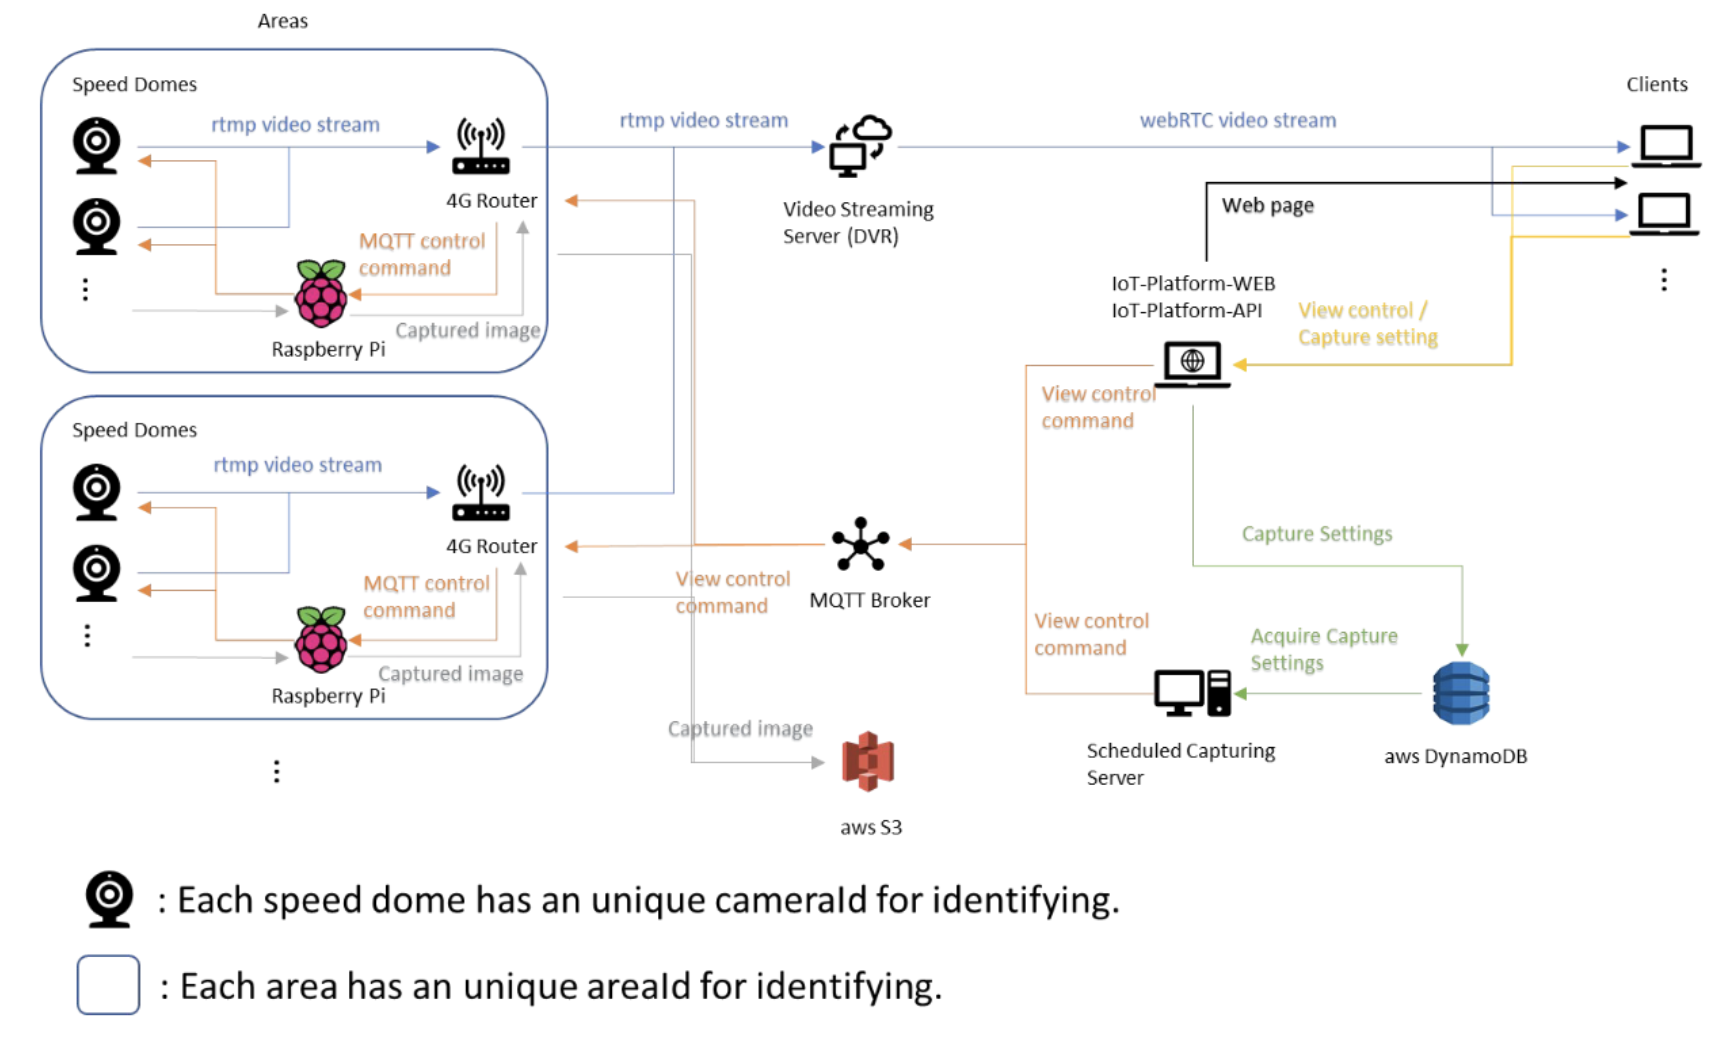
\includegraphics[width=\textwidth]{figsrc/Previous-IPcam-system-chart.png}
%     \caption{Streaming System overview.\label{fig:Previous-IPcam-system-chart}}
% \end{figure}


% \section{Binarization}



% In recognition of printed scores, the color information, namely R/G/B or R/G/B/A vectors, is not useful. Instead, only the intensity information is considered for recognition, so gray-scaled images are always used as the raw input. Furthermore, people always determine if each pixel is background (white) or foreground (black) in advance, and hence the binarization is included in most applications of OMR.

% In Pinto's research~\cite{agri-wiki}, two kinds of binarization methods were introduced depending on whether the binarization threshold is locally adjustable. The simplest way is applying a constant threshold to all pixels in the image, which is called \emph{global thresholding}. The global threshold can be obtained by finding a value that maximizes the variance~\cite{Otsu:1979:ATSMfGLH} between foreground and background pixels, preserves the most edge information~\cite{Chen:2008:ADTIBMboED}, or maximizes the similarity between the binarized image and the original image~\cite{Huang:1995:ITbMtMoF,Tsai:1995:AFTSPfMaUH}. However, it cannot be expected that the intensity in different small regions is constant over the document, and a constant threshold might not work at a different intensity level. In particular, near the boundary of a page in a book, the image might show a gradient-like difference in terms of the average intensity as compared to the region far from the book spine (Fig.~\ref{fig:bookspine}). To deal with such situations, the choice of the threshold should be determined by local information (nearby pixels)~\cite{Bernsen:2005:DToGLI}, which is called \emph{local thresholding}. In general, global thresholding is easier to be implemented, while local thresholding is more adaptive and robust.

% \begin{figure}[ht]
%     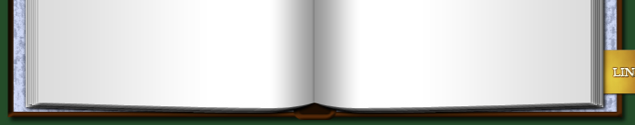
\includegraphics[width=\textwidth]{bookspine}
%     \caption{Example of the gray-scale image near the book spine\label{fig:bookspine}.}
% \end{figure}

% \section{Staff Detection and Removal}

% Dalitz et al.~\cite{Dalitz:2008:CSoSRA} introduced a systematic way for testing the staff removal algorithms. A dataset was generated from a set of ideal score images with the deformation methods listed in Table.~\ref{table:deformation}. The deformation algorithms and the CVC-MUSCIMA dataset are made openly available by Forns et al.~\cite{Forns:2012:CVC-MUSCIMA}.

% \begin{table}[ht]
%     %\hspace{-.5in}
%     \begin{tabular}{|c|c|c|}
%         \hline
%         {\bf Deformation} & {\bf Type} & {\bf Parameter Description} \\
%         \hline
%         Curvature & deterministic & height/width ratio of sine curve \\
%         \hline
%         Typeset Emulation & both & \parbox[c]{9cm}{gap width, maximal height and variance of vertical shift} \\
%         \hline
%         Line Interruptions & random & \parbox[c]{9cm}{interruption frequency, maximal width and variance of gap width} \\
%         \hline
%         Thickness Variation & random & \parbox[c]{9cm}{Markov chain stationary distribution and inertia factor} \\
%         \hline
%         $y$-variation & random & \parbox[c]{9cm}{Markov chain stationary distribution and inertia factor} \\
%         \hline
%         Degradation & random & \parbox[c]{9cm}{emulating local distortions suggested by Kanungo et al.} \\
%         \hline
%         White Speckles & random & \parbox[c]{9cm}{speckle frequency, random walk length and smoothing factor} \\
%         \hline
%     \end{tabular}
%     \caption{Deformation Methods\label{table:deformation}.}
% \end{table}



